% Lecture Template for ME3001-001-Tristan Hill - Spring 2017 - Fall 2017
% 
% Mechanical Engineering Analysis with MATLAB
%
% Introduction to Analysis

% Document settings
\documentclass[11pt]{article}
\usepackage[margin=1in]{geometry}
\usepackage[pdftex]{graphicx}
\usepackage{multirow}
\usepackage{setspace}
\usepackage{hyperref}
\usepackage{color,soul}
\usepackage{fancyvrb}
\usepackage{framed}
\usepackage{wasysym}
\usepackage{multicol}
\usepackage{ amssymb }



\pagestyle{plain}
\setlength\parindent{0pt}
\hypersetup{
    bookmarks=true,         % show bookmarks bar?
    unicode=false,          % non-Latin characters in Acrobat’s bookmarks
    pdftoolbar=true,        % show Acrobat’s toolbar?
    pdfmenubar=true,        % show Acrobat’s menu?
    pdffitwindow=false,     % window fit to page when opened
    pdfstartview={FitH},    % fits the width of the page to the window
    pdftitle={My title},    % title
    pdfauthor={Author},     % author
    pdfsubject={Subject},   % subject of the document
    pdfcreator={Creator},   % creator of the document
    pdfproducer={Producer}, % producer of the document
    pdfkeywords={keyword1} {key2} {key3}, % list of keywords
    pdfnewwindow=true,      % links in new window
    colorlinks=true,       % false: boxed links; true: colored links
    linkcolor=red,          % color of internal links (change box color with linkbordercolor)
    citecolor=green,        % color of links to bibliography
    filecolor=magenta,      % color of file links
    urlcolor=blue           % color of external links
}

% assignment number 
\newcommand{\NUM}{1 } 
\newcommand{\VSpaceSize}{2mm} 
\newcommand{\HSpaceSize}{2mm} 

\newcommand{\Lagr}{\mathcal{L}}

\definecolor{mygray}{rgb}{.6, .6, .6}

\setulcolor{red} 
\setstcolor{green} 
\sethlcolor{mygray} 

\begin{document}

\textbf{ \LARGE ME 3050 Lecture - Introduction to Analysis} \vspace{3mm}\\
\textbf{ \hspace*{5mm}Tristan W. Hill - Tennessee Technological University - Spring 2020 } \vspace{3mm}\\

\begin{itemize}


	\item \textbf{ \LARGE We spent the last two weeks deriving differential equations. } \\

\item \textbf{ \LARGE Now What?}\\
			

\vspace{120mm}
\item \textbf{ \LARGE Lecture This Week}
\Large
\begin{itemize}
	\item Trial Solution - 1$^{st}$ 2$^{nd}$ Order - Free Response\\
	\item Trial Solution - $f(t)$ - General Forms\\
	\item {\it re}Introduce Laplace Transform - $\Lagr\{y(t)\}$
\end{itemize}


	\newpage
\item \textbf{ \LARGE Consider the system shown below. Make? Model?} \vspace{3mm}\\
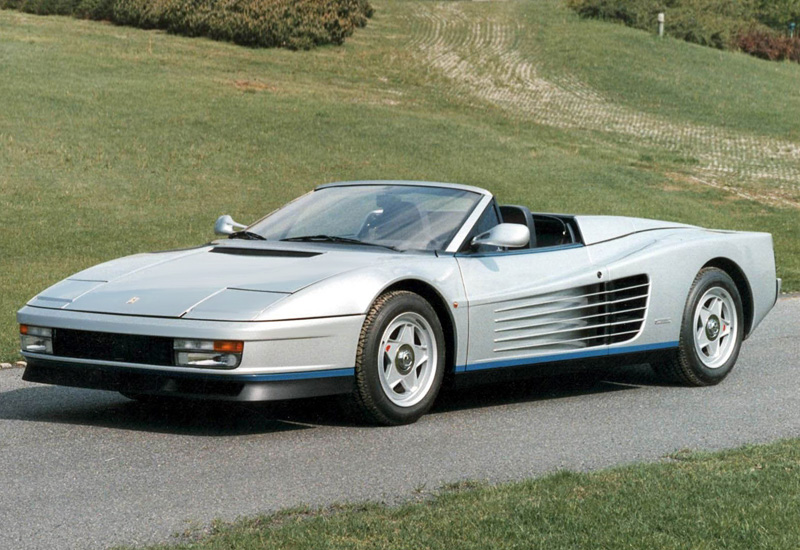
\includegraphics[scale=0.5]{ferrari.jpg}
	
		

	\newpage
\item \textbf{ \LARGE Response of 1$^{st}$ Order System with \underline{Constant Input}}



	\newpage
\item \textbf{ \LARGE Response of 2$^{nd}$ Order System with \underline{Constant Input}}

	\end{itemize}

\end{document}



